%\documentclass[preprint,tightenlines,showpacs,showkeys,floatfix,
%nofootinbib,superscriptaddress,fleqn]{revtex4} 
\documentclass[tightenlines,floatfix,nofootinbib,superscriptaddress,fleqn]{revtex4-2}  
%\documentclass[aps,epsfig,tightlines,fleqn]{revtex4}
\usepackage{kotex}
\usepackage[HWP]{dhucs-interword}
\usepackage[dvips]{color}
\usepackage{graphicx}
\usepackage{bm}
%\usepackage{fancyhdr}
%\usepackage{dcolumn}
\usepackage{defcolor}
\usepackage{amsmath}
\usepackage{amsfonts}
\usepackage{amssymb}
\usepackage{amscd}
\usepackage{amsthm}
\usepackage[utf8]{inputenc}
%\pagestyle{fancy}

\begin{document}

\title{\Large 2020년 2학기 물리학 II}

\author{Byeong-woo Han} 
\email{12191964@inha.edu}
\affiliation{Hadron Theory Group, Department of Physics,
  Inha  University, Incheon 22212, Republic of Korea }
  \author{Hui-Jae Lee} 
  \email{hjlee6674@inha.edu}
  \affiliation{Hadron Theory Group, Department of Physics,
    Inha  University, Incheon 22212, Republic of Korea }
  \author{김현철\footnote{Office: 5S-436D (면담시간 매주
  수요일-16:15$\sim$19:00)}} 
\email{hchkim@inha.ac.kr}
\affiliation{Hadron Theory Group, Department of Physics,
Inha  University, Incheon 22212, Republic of Korea }
\date{Autumn Semester, 2020}


\maketitle

{\color{red} {\bf Due date:} 2020년 9월 14일  15:25-16:15 }
\vspace{1.cm}

\section*{\large Quiz 5}
\noindent {\bf 문제 1 [20pt].} 반지름이 $r$이고 길이가 $L$인 원통형
구리 도선이 있다. 부피를 일정하게 유지한 채로 이 도선을 늘려 길이가 두
배가 되었다면, 저항은 처음의 몇 배가 되었는가? 
\vspace{0.5cm}

\noindent{\bf 풀이 : }
길이가 $L$이고 단면적이 $A$인 도선의 저항 $R$은 길이에 비례하고 단면적에 반비례한다. 즉,
\begin{align}
  R=\rho\frac{L}{A}
\end{align}
이고 $\rho$은 도선의 비저항이다. 처음 저항을 $R_0$, 처음 반지름을 $r_0$라 하자. 
$R_0$는
\begin{align}
  R_0 = \rho\frac{L}{\pi r^2_0}
\end{align}
로 쓸 수 있는데 길이를 2배로 늘리고 부피를 유지했다면 반지름이 변했을 것이다. 변한 반지름 $r$은
부피를 유지했다는 사실로부터 얻을 수 있다.
\begin{align}
  \pi r^2_0 L = \pi r^2(2L)\Longrightarrow r = \frac{1}{\sqrt{2}}r_0.
\end{align}
따라서 변한 저항 $R$은 다음과 같다.
\begin{align}
  R = \rho\frac{2L}{\pi r^2}=\rho\frac{4L}{\pi r_0^2}=4R_0.
\end{align}
길이를 2배로 늘리고 부피를 유지하면 저항은 4배 증가한다.
\vspace{0.5cm}

\noindent {\bf 문제 2 [20pt].} 반지름이 $a$인 도체공을 중심이 같고
반지름이 $b$ ($b>a$)이고 비저항이 $\rho$인 물질로 만들어진 공을 감싸고
있다. 이 두 공 사이의 저항을 구하여라.  

\vspace{0.5cm}

\noindent{\bf 풀이 : }
두 공 사이의 저항을 구하기 위해 먼저 두 공 사이에 놓여진 미소 구껍질을 생각하자. 이 미소 구껍질은
두 공과 중심이 같고 반지름이 $r$이며 두께는 $dr$이다. 이 미소 구껍질 사이의 미소 저항을 구한다면,
미소 저항을 거리 $a$부터 $b$까지 적분하여 반지름이 $a$인 공과 반지름이 $b$인 공 사이의 저항을
알아낼 수 있다. 미소 구껍질의 면적은 $4\pi r^2$이므로 미소저항 $dR$은
\begin{align}
  dR = \rho\frac{dr}{4\pi r^2}
\end{align}
으로 쓸 수 있다. 양변을 적분하면
\begin{align}
  \begin{split}
    \int dR &= \int^b_a  \rho\frac{dr}{4\pi r^2}
    =\frac{\rho}{4\pi}\int^b_a\frac{1}{r^2}\,dr
    =\frac{\rho}{4\pi}\left.\left(-\frac{1}{r}\right)\right|^{b}_{a}
    =\frac{\rho}{4\pi}\left(
      -\frac{1}{b}+\frac{1}{a}
      \right) \\
    &= \frac{\rho(b-a)}{4\pi ab}
    \end{split}
\end{align}
을 얻는다. 즉, 두 공 사이의 저항은 $\frac{\rho(b-a)}{4\pi ab}$이다.
\vspace{0.5cm}

\noindent {\bf 문제 3 [20pt].} 
저항값이 $R$인 저항이 달려 있는 단일고리
회로에 5.0 A의 전류가 흐르고 있다. 여기에 직렬로 저항이 $5.0\,\Omega$인
저항소자를 직렬로 회로에 연결하자 전류가 $4.0$ A로 낮아졌다. $R$ 값을
구하여라.   

\vspace{0.5cm}

\noindent{\bf 풀이 : }
처음 전압, 전류, 저항을 각각 $V$, $I=5.0$ A, $R$이라고 하면 옴의 법칙에 의해 다음이 성립한다.
\begin{align}\label{eq:3-1}
  V = IR.
\end{align}
여기에 저항 $R'=5.0\,\mathrm{\Omega}$를 직렬로 연결하였으므로 변한 전압 $V'$와 전류 $I'=4.0$
A는 다시 옴의 법칙을 만족한다. 즉,
\begin{align}\label{eq:3-2}
  V' = I'(R+R')
\end{align} 
이다. 저항을 추가로 연결한다고 회로의 전압이 달라지지는 않으므로 $V=V'$이고 식~(\ref{eq:3-1})과
식~\eqref{eq:3-2}로부터
\begin{align}
  IR=I'(R+R')\Longrightarrow
  R = \frac{I'}{I+I'}R'=\frac{4.0~\mathrm{A}}{5.0~\mathrm{A}+4.0~\mathrm{A}}
  (5.0~\mathrm{\Omega})=2.2~\mathrm{\Omega}
\end{align}
를 얻는다. 따라서 처음 저항 $R$은 $2.2~\mathrm{\Omega}$이다.
\vspace{0.5cm}

\noindent {\bf 문제 4 [20pt].} 
그림~\ref{fig:1}은 번개가 치는 날 나무 옆에 있으면 왜 안 되는지
보여준다. 나무에 낙뢰가 떨어지면, 나무껍질을 타고 번개전류가 흐른다.
그런데 번개전류가 나무껍질 중에서 물기가 없는 부분에 도달하면 전류 중
일부분이 습기가 높은 공기 중으로 새어나가 옆에 서 있는 사람에게로
흘러간다. 사람은 습도가 높은 공기에 비해 전도도가 훨씬 높아서
그렇다. 이때 나무와 사람 사이의 거리가 $d$이고, 사람의 키가 $h$라고
하면, 번개전류의 일부분이 나무에서 사람으로 $d$만큼 거리를 흐르고,
다시 사람을 따라 $h$만큼 높이를 흘러 바닥으로 간다고 하자. 만약에
$d/h=0.400$이고, 총전류는 $I=5\,000$ A라고 하면, 사람을 지나는 전류는
얼마인가? 

\begin{figure}[htp]
  \centering
  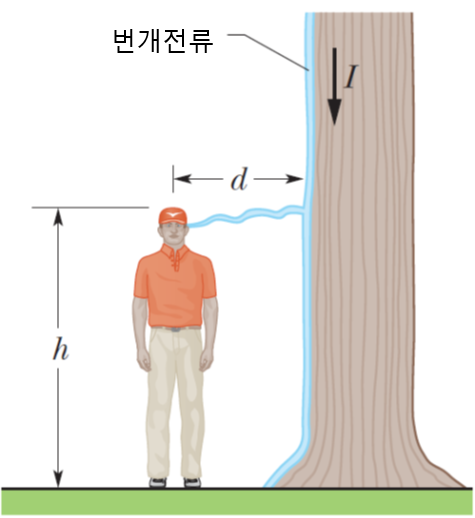
\includegraphics[scale=0.45]{qfig5-20220914-1.png}
  \caption{\textbf{문제 4}}
  \label{fig:1}
\end{figure}

\vspace{1.cm}

\noindent {\bf 풀이 :}
저항 $R$은
\begin{align}
  R=\rho\frac{A}{l}=\frac{1}{\sigma}\frac{A}{l}
\end{align}
이고 이동한 거리에 반비례한다.
사람의 전기전도도가 훨씬 높으므로 사람의 저항 $R_{h}$을 $0$라고 가정하자. 
또한 나무껍질의 습도가 높은 공기를 타고 전류가 내려가므로 전기전도도는
$\sigma$로 같다. 따라서  넓이 $A$는 매우 작으므로 같다고 가정한다.
$d$로 이동한 거리가 수평이라고 가정할 때, 먼저 거리가 $h$인 저항$R_h$와
거리가 $d$인 저항$R_d$와의 비는 다음과 같다.
\begin{align}
  \frac{R_h}{R_d}=\frac{d}{h}=0.400
\end{align}
이제 사람을 지나는 전류를 구하기 위해 옴의 법칙을 이용하자. 처음 전압을
$V$, 땅의 전압을 $0~\mathrm{V}$라 가정하고 사람을 따라 땅까지
흐르는 전류를 $I_d$, 나무껍질을 따라 땅까지 흐르는 전류를 $I_h$라고 하자.
전하량 보존법칙에 의해서 다음이 성립한다.
\begin{align}
  I=I_d+I_h.
  \label{eq:4-1}
\end{align}
또한, 두 저항이 병렬로 연결되있으모로, 옴의 법칙에 의해 다음이 성립한다.
\begin{align}
  \begin{split}
   &I_h=\frac{V}{R_h},\\
   &I_d=\frac{V}{R_d}.
   \label{eq:4-2}
  \end{split}
\end{align}
식~(\ref{eq:4-2})을 식~(\ref{eq:4-1})에 대입하면 다음과 같은 결과를 
얻을 수 있다.
\begin{align}
  \begin{split}
   I&=V\left(\frac{1}{R_d}+\frac{1}{R_h}\right)\\
   &=\frac{V}{R_h}\left(1+\frac{R_h}{R_d}\right)\\
  \end{split}
\end{align}
식~(\ref{eq:4-2})과 $I=5\,000~\mathrm{A}$, ${R_h}/{R_d}=0.400$을 대입하면
\begin{align}
   5000~\mathrm{A}=1.40I_h\Longrightarrow
   I_h=\frac{5000}{1.40}~\mathrm{A}
\end{align}
이다. 즉, 사람에게 흐르는 전류 $I_h$는
\begin{align}
  I_h = 3570~\mathrm{A}
\end{align}
으로 사람에게는 $3570~\mathrm{A}$만큼의 전류가 흐르게 된다.
%을 얻고 이를 식~(\ref{eq:4-1})에 대입하면
%\begin{align}
%  \begin{split}
%    &5000=I_d+\frac{5000}{1.400}\\
%    &I_d=5000\left(1-\frac{1}{1.400}\right)\\
%    &\quad\approx 3570~\mathrm{A}
%  \end{split}
%\end{align}
%이다.

\vspace{1.cm}

\noindent {\bf 문제 5 [20pt].} 
그림~\ref{fig:2}처럼 $a$와 $b$ 사이에 똑같이 생긴 저항 다섯 개가
연결되어 있을 때, 등가저항을 구하여라. 
\begin{figure}[htp]
  \centering
  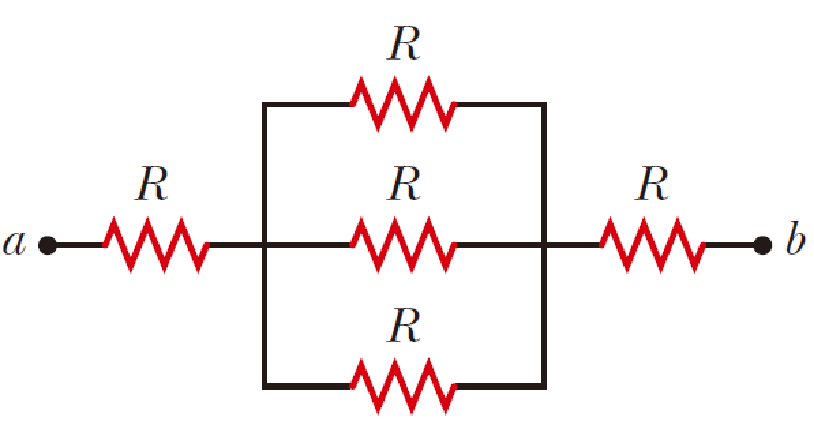
\includegraphics[scale=0.45]{qfig5-20220914-2.pdf}
  \caption{\textbf{문제 5}}
  \label{fig:2}
\end{figure}
\vspace{1.cm}

\noindent {\bf 풀이 :}
먼저 회로의 가운데에 있는 세 병렬저항들의 합성저항을 구하자.
세 개의 병렬저항 $R_j$의 합성저항 $R_{eq}$는 다음과 같이 쓸 수 있다.
\begin{align}
  \frac{1}{R_{eq}}=\sum^{N}_{j=1}\frac{1}{R_j}.
\end{align}
여기서, $N=3$, $R_1=R_2=R_3=R$이므로
\begin{align}
  \begin{split}
   \frac{1}{R_{eq}}&=\sum^{N}_{j=1}\frac{1}{R_j}\\
   &=\frac{1}{R}+\frac{1}{R}+\frac{1}{R}\\
   &=\frac{3}{R} 
  \end{split}
\end{align}
이다. 따라서
\begin{align}
  R_{eq}=\frac{R}{3}
\end{align}
를 얻는다. 이제 전체 합성저항들을 구하자. 가운데 합성저항이
양 옆의 저항과 직렬로 연결되어 있으므로 세 직렬저항 $R'_j$의 합성저항
$R'_{eq}$는 다음과 같이 쓸 수 있다.
\begin{align}
  R'_{eq}=\sum^N_{j=1}R'_j.
\end{align}
여기서, $N=3$, $R'_1=R'_3=R$, $R'_2=R_{eq}=R/3$이므로,
\begin{align}
  \begin{split}
    R'_{eq}&=R+\frac{R}{3}+R\\
    &=\frac{7}{3}R
  \end{split}
\end{align}
이다. 따라서 총 합성저항 $R'_{eq}$는
\begin{align}
  R'_{eq}=\frac{7}{3}R
\end{align}
이다.
\end{document}